\documentclass[11pt,letterpaper]{article}

\usepackage[margin=1in]{geometry}
\usepackage[T1]{fontenc}
\usepackage[utf8]{inputenc}
\usepackage{microtype}
\usepackage{amsmath,amssymb}
\usepackage{booktabs}
\usepackage{graphicx}
\usepackage{caption}
\usepackage{authblk}
\usepackage{enumitem}
\usepackage[hyphens]{url}
\usepackage{xcolor}
\usepackage[round,authoryear]{natbib}
\usepackage{hyperref}

\hypersetup{
  pdftitle={High-ROIC Compounding under AAOIFI Debt Limits: An Exploratory Backtest of Halal ROIC Reinvestment, 2022-2024},
  pdfauthor={Rao Abdul Hadi},
  pdfsubject={Halal equity investing, ROIC, reinvestment, AAOIFI screens},
  pdfkeywords={ROIC, reinvestment, AAOIFI, Sharia-compliant equities, quality factor, backtest},
  colorlinks=true,
  citecolor=blue,
  linkcolor=blue,
  urlcolor=blue
}

\captionsetup{font=small,labelfont=bf,skip=6pt}
\setlength{\parindent}{1.5em}
\setlength{\parskip}{0pt}
\setlist[itemize]{leftmargin=1.5em,itemsep=0.2em,topsep=0.35em}
\setlist[enumerate]{leftmargin=1.5em,itemsep=0.2em,topsep=0.35em}

\renewcommand\Authfont{\normalsize}
\renewcommand\Affilfont{\small}
\setlength{\affilsep}{0.6em}

\title{\textbf{High-ROIC Compounding under AAOIFI Debt Limits:\\
An Exploratory Backtest of Halal ROIC Reinvestment, 2022--2024}}

\author[1]{Rao Abdul Hadi\thanks{Corresponding author. Email: \href{mailto:raoabdulhadi952@gmail.com}{raoabdulhadi952@gmail.com}.}}
\affil[1]{Monterey Finance, Halal Quant Research Lab}

\date{September 2026}

\begin{document}
\maketitle

\begin{abstract}
\noindent
This paper asks a simple question. After Islamic business and leverage screens have been applied, do firms that earn a high return on invested capital and put a large share of those earnings back into the business compound faster than the broad market? I start from the S\&P~500, drop banned activities and names that fail AAOIFI financial-ratio tests, keep companies with ROIC above 15\% whose reinvestment rate sits in the top half of that pool, and own the survivors in proportion to market cap. From 31~October~2022 through 30~December~2024 the book returned 39.6\% compound annual growth, against 22.9\% for the S\&P~500 (SPY) and 27.4\% for a Halal large-cap ETF (SPUS). Inside the high-ROIC pool, high reinvestment beat low reinvestment (43.2\% versus 28.7\% CAGR). Sorting on ROIC alone was much noisier: the top quintile did not cleanly beat the bottom. The live portfolio is still a concentrated Halal mega-cap technology and platform book. Technology plus communication services average about 82\% of GICS weight. A robustness sleeve limited to SaaS, healthcare, and med-tech returned 27.6\% CAGR, roughly in line with SPUS and below the unrestricted compounder book. The sample is short, the fundamental data come from Yahoo annual statements, and I do not estimate a sector-neutral twin. The numbers should be read as an exploratory backtest, not as a forecast or a live-return target.
\end{abstract}

\noindent\textbf{Keywords:}
ROIC; reinvestment rate; AAOIFI; Sharia-compliant equities; quality factor; compounding; backtest.

\noindent\textbf{JEL classification:} G11, G12, Z12.

\noindent\textbf{Code:}
Replication notebook and figures are in the Monterey Finance repository,
\url{https://github.com/regional-specter/Monterey-Finance},
under \path{Research/papers/02-roic-engine/}.

\section{Introduction}

Return on invested capital (ROIC) is a standard way to ask how hard each dollar of operating capital works. Reinvestment rate asks what share of those profits is put back into the firm rather than paid out. In the quality literature, businesses that earn high returns and reinvest at those returns are the ones that should compound book value, and eventually price, faster than the market \citep{damodaran2007,novymarx2013,asness2019}. Islamic equity screens add a second filter. AAOIFI financial-ratio limits cap interest-bearing debt, cash, and receivables relative to market value, and a separate activity screen removes banks, conventional insurance, alcohol, tobacco, gambling, weapons, and similar businesses \citep{aaoifi21}. The economic hope is that those caps already strip out highly indebted firms, so that among what remains, ROIC and reinvestment are cleaner signals.

That hope is not automatic. Sharia screens change the sector mix. They tend to cut financials and some utilities, and they leave a larger weight in technology, healthcare, and other operating businesses. Any backtest that looks good after those screens may simply be riding the same mega-cap platform names that dominated 2023 and 2024. The original motivation for this study was compounding in capital-light sectors (SaaS, healthcare, and med-tech), where research and development and other intangible spending matter more than plant and equipment. Those sectors need to be checked, not assumed.

The live rule tested here is therefore narrow. After banned businesses and the AAOIFI debt, cash, and receivables tests, keep names with ROIC above 15\%, positive NOPAT, positive invested capital, and a positive reinvestment rate, then keep the top half of that list by reinvestment rate and cap-weight it. The question is whether that book holds up against both an all-stock benchmark (SPY) and a Halal large-cap benchmark (SPUS) over the window for which the data actually support a live portfolio.

It does, on headline returns. It also takes more drawdown than either benchmark, it is heavily concentrated in a handful of platform names, and the capital-light robustness sleeve does not beat the main book. ROIC quintiles inside the Halal universe are not monotonic. The cleaner split is the one the live rule actually uses: high versus low reinvestment among names that already clear the 15\% ROIC floor. I treat that as supporting evidence for the compounding story, not as proof that the story survives a full market cycle.

The rest of the paper is organized as follows. Section~\ref{sec:data} describes the universe, screens, and factor definitions. Section~\ref{sec:rules} states the portfolio rules. Section~\ref{sec:results} reports live-window performance, calendar years, drawdowns, and the two diagnostic sorts. Section~\ref{sec:attrib} looks at alpha, beta, and sector mix. Section~\ref{sec:limits} covers turnover, purification, data limits, and what would be required before treating this as a live mandate. Section~\ref{sec:conc} concludes.

\section{Data, screens, and factor definitions}
\label{sec:data}

\subsection{Universe}

The starting list is the current S\&P~500 (503 tickers). A one-time activity screen removes 64 names, leaving 439 sector-eligible stocks. Financial-ratio screens then re-run at every month-end on filings that would have been known as of that date. I use \texttt{filed\_date} when it is available, and otherwise the report date plus a 90-day publication lag.

The requested price sample is 1~January~2019 through 31~December~2024. Yahoo annual statements do not go back far enough for a 2019 start. The first date with usable ROIC and reinvestment metrics is 30~November~2021. Performance statistics begin on the first day the strategy actually holds stocks, 31~October~2022, and run through 30~December~2024 (544 trading days). Days before that first invested date are omitted, not filled with zeros.

Yahoo had no in-sample price history for Q, SNDK, and FDXF. Those names are skipped where data are missing. Baker Hughes (BKR) hit a cache lock once during download and is skipped on that pull.

\subsection{Screening standard}

The financial screens follow AAOIFI ratios, not the Dow Jones Islamic Market (DJIM) thresholds \citep{aaoifi21,derigs2008}. The debt rule in this test is total debt below 30\% of trailing 24-month market cap, together with the library's cash and receivables screens. Compliance is a hard constraint. A name that fails on a rebalance date is not held.

SPUS (SP Funds S\&P~500 Sharia Industry Exclusions) is the Halal index comparison. It is a cap-weighted, industry-exclusion ETF. It is not identical to a pure AAOIFI financial-ratio index, so beating SPUS is not the same as beating ``the'' Sharia market. SPY is the all-stock benchmark.

Table~\ref{tab:universe} summarizes the design choices.

\begin{table}[htbp]
\centering
\caption{Universe, screens, and sample.}
\label{tab:universe}
\begin{tabular}{ll}
\toprule
Item & Choice \\
\midrule
Target factors & ROIC $> 15\%$; reinvestment rate in top half of that pool \\
Starting universe & Current S\&P~500 list (503 tickers) \\
After banned-business screen & 439 tickers (64 removed) \\
Focus-sector tags (diagnostic) & SaaS 40, healthcare 25, med-tech 33, other 341 \\
Screening standard & AAOIFI financial ratios, not DJIM \\
Halal benchmark & SPUS (SP Funds S\&P~500 Sharia Industry Exclusions) \\
All-stock benchmark & SPY (S\&P~500) \\
Sample requested & 1~Jan~2019 -- 31~Dec~2024 \\
First metrics date & 30~Nov~2021 \\
Live window used for stats & 31~Oct~2022 -- 30~Dec~2024 (544 trading days) \\
\bottomrule
\end{tabular}
\end{table}

\subsection{ROIC and reinvestment}

ROIC is net operating profit after tax divided by invested capital:
\[
\mathrm{ROIC} = \frac{\mathrm{NOPAT}}{\mathrm{Invested\ capital}},
\qquad
\mathrm{NOPAT} = \mathrm{EBIT} \times (1 - \tau),
\]
where $\tau$ is the effective tax rate when it is usable and 21\% otherwise. Names with ROIC above 500\% are dropped as denominator errors.

Reinvestment rate measures how much of NOPAT is put back into the business:
\[
\mathrm{Reinvestment\ rate}
= \frac{\mathrm{CapEx} - \mathrm{D\&A} + \Delta\mathrm{NWC} + \mathrm{R\&D}}{\mathrm{NOPAT}}.
\]
Research and development is counted as reinvestment so that capital-light software and med-tech names are not scored as low reinvestment simply because they spend little on factories. That choice follows the usual treatment of intangible investment in quality and compounding work \citep{damodaran2007,peters2017}. Fundamentals come from yfinance annual income, balance-sheet, and cash-flow statements, lagged 90 days.

I do not claim that AAOIFI screens create a ROIC premium by themselves. The live window is short, mega-cap heavy, and partly overlapping with the 2023--2024 platform boom. The capital-light robustness sleeve is there to test whether SaaS, healthcare, and med-tech compounders persist. It is not the primary live rule.

\section{Portfolio rules}
\label{sec:rules}

Rules are applied at month-end with no look-ahead. There is no intra-month stop-loss and no single-name position cap beyond cap-weighting.

\subsection{Pipeline at each month-end}

\begin{enumerate}
  \item Start from the sector-eligible S\&P~500 list (439 names).
  \item Drop names that fail the AAOIFI debt, cash, or receivables screens on filings known as of that date.
  \item Compute ROIC and reinvestment rate from annual statements.
  \item Require ROIC $> 15\%$, positive NOPAT, positive invested capital, and reinvestment rate $> 0$. Keep the top half of that Halal list by reinvestment rate (\texttt{KEEP\_QUANTILE} $= 0.50$).
  \item Cap-weight by market cap. No equal-weight, no inverse-volatility, and no optimizer.
  \item Repeat at month-end (\texttt{REBALANCE\_FREQ} $=$ \texttt{ME}).
\end{enumerate}

If fewer than 20 names survive (\texttt{MIN\_HOLDINGS}), that month is skipped and the book stays in cash. Cash months are treated as missing, not as a 0\% return. Statistics start on the first invested date, not on the 2019 calendar start.

\begin{table}[htbp]
\centering
\caption{Entry, exit, and risk limits.}
\label{tab:rules}
\small
\begin{tabular}{lp{0.62\textwidth}}
\toprule
Rule & Specification \\
\midrule
Entry & Halal, ROIC $> 15\%$, positive reinvestment, top half by reinvestment \\
Exit & Sold at the next month-end if the name fails AAOIFI, loses the ROIC/reinvestment test, or drops out of the top half \\
Intra-month stop-loss & None \\
Position cap & None beyond cap-weight \\
Cash when thin & Skip the month if holdings $< 20$ \\
Robustness twin & Same screen, then keep only SaaS / healthcare / med-tech \\
\bottomrule
\end{tabular}
\end{table}

At the last rebalance (31~December~2024), Nvidia was 20.4\% of the book, Microsoft 19.0\%, and the two Alphabet share classes together were about 28.7\%. That is a concentrated mega-cap book by construction. A 5\% or 8\% name cap would change both risk and 2023--2024 return. I leave that for a follow-up rather than rewriting the live rule after seeing the weights.

\subsection{Holdings through time}

Median live book size is 51 names (minimum 5 in the early build, maximum 64). At a typical month the funnel is roughly 418 names with fundamentals, 100 Halal names with ROIC above 15\% and positive reinvestment, and 50 actually bought. About half of the high-ROIC pool sits in the tagged SaaS, healthcare, and med-tech buckets, but cap-weighting still leaves most of the money in ``other'' mega-caps.

\begin{figure}[htbp]
\centering

\includegraphics[width=0.88\textwidth]{figures/holdings-count.png}
\caption{Number of names held at each month-end. The book ramps from a thin early window to a stable sleeve of about 50 names through 2024.}
\label{fig:holdings}
\end{figure}

Sharia status, ROIC, and reinvestment rank are re-checked every month. A held name that fails is exited at that rebalance. It is not left in the book pending a discretionary review.

On 31~December~2024 the watchlist looked as follows. Held names included NVDA, MSFT, GOOGL, ADBE, and LLY: all Halal-ok, all in the top half by reinvestment among the 99-name high-ROIC pool. Apple passed the screens with ROIC of 57\% but ranked 58 of 99 on reinvestment, so it was treated as a cash-rich harvester on this metric and not bought. Several med-tech and SaaS names (ISRG, SYK, TMO, INTU, NOW, ORCL, and others) sat below the 15\% ROIC floor on Yahoo filings despite strong reinvestment rates. UNH and ABBV had negative reinvestment that month.

GOOG and GOOGL were both held as separate lines. Cap-weighting two share classes of the same company inflates Alphabet relative to a single-listing index. That is a construction error to fix in a follow-up.

Many capital-light med-tech names failed the 15\% ROIC floor in this data. That matters for the original sector story. The reinvestment sort worked inside the high-ROIC pool, but med-tech did not dominate the book the way a SaaS/healthcare/med-tech compounding hypothesis would have suggested.

\section{Empirical performance}
\label{sec:results}

All headline numbers use the live window only: 31~October~2022 through 30~December~2024. Sharpe and Sortino use a 2\% risk-free rate. Maximum drawdown is peak-to-trough on the growth curve.

\subsection{Headline results}

\begin{table}[htbp]
\centering
\caption{Live-window performance, 31~Oct~2022 -- 30~Dec~2024.}
\label{tab:perf}
\small
\begin{tabular}{lrrrrrr}
\toprule
Book & CAGR & Vol. & Sharpe & Sortino & Max DD & Calmar \\
\midrule
Halal ROIC compounders                    & 39.57\% & 19.48\% & 1.71 & 2.57 & $-15.33\%$ & 2.58 \\
Compounders (SaaS / HC / med-tech)        & 27.61\% & 17.48\% & 1.37 & 1.97 & $-15.07\%$ & 1.83 \\
S\&P~500 (SPY)                            & 22.94\% & 13.92\% & 1.41 & 2.13 & $-9.97\%$  & 2.30 \\
Halal (SPUS)                              & 27.35\% & 16.20\% & 1.45 & 2.24 & $-11.46\%$ & 2.39 \\
\bottomrule
\end{tabular}
\end{table}

The compounder book beat both benchmarks on CAGR, Sharpe, Sortino, and Calmar. It took a deeper drawdown than SPY ($-15.3\%$ versus $-10.0\%$) and SPUS ($-11.5\%$). The capital-light robustness sleeve matched SPUS on CAGR (27.6\% versus 27.4\%) with a similar drawdown. It did not beat the broad compounder book.

These CAGRs are annualized figures from a mega-cap bull market. They are not a forecast of 40\% a year.

\begin{figure}[htbp]
\centering

\includegraphics[width=0.88\textwidth]{figures/equity-curves.png}
\caption{Growth of \$1 in the live window. The main compounder book leads. The capital-light sleeve tracks closer to SPUS.}
\label{fig:equity}
\end{figure}

\subsection{Calendar years}

\begin{table}[htbp]
\centering
\caption{Calendar-year total returns inside the live window.}
\label{tab:calendar}
\begin{tabular}{lrrr}
\toprule
Year & Halal ROIC compounders & S\&P~500 & Halal (SPUS) \\
\midrule
2022 & $-2.28\%$ & $-1.24\%$ & $-1.64\%$ \\
2023 & 56.67\% & 26.18\% & 34.20\% \\
2024 & 34.16\% & 25.34\% & 27.67\% \\
\bottomrule
\end{tabular}
\end{table}

The compounder book led strongly in 2023 and 2024. 2022 is only a partial year (live from late October), and all three books were slightly negative in that stub.

\begin{figure}[htbp]
\centering

\includegraphics[width=0.88\textwidth]{figures/calendar-year-returns.png}
\caption{Calendar-year returns. The compounder book is the tallest bar in 2023 and 2024.}
\label{fig:calendar}
\end{figure}

\begin{figure}[htbp]
\centering

\includegraphics[width=0.88\textwidth]{figures/rolling-excess.png}
\caption{Rolling 12-month excess return versus SPY. Excess stayed positive through most of the live window.}
\label{fig:excess}
\end{figure}

\subsection{Drawdowns}

\begin{figure}[htbp]
\centering

\includegraphics[width=0.88\textwidth]{figures/drawdowns.png}
\caption{Drawdowns in the live window. The compounder book dips with Halal and technology names and takes a deeper trough than SPY in mid-to-late 2024.}
\label{fig:dd}
\end{figure}

The compounder book and SPUS move together in late 2023 and 2024. SPY's drawdowns are shallower. That pattern is consistent with a Halal mega-cap platform book, not with a defensive quality sleeve.

\subsection{Does higher ROIC actually compound?}

Two cuts inside the Halal universe test the factor logic.

\paragraph{ROIC quintiles.}
Cap-weight five buckets by ROIC. Q1 is the highest ROIC and Q5 is the lowest.

\begin{table}[htbp]
\centering
\caption{Cap-weighted ROIC quintiles inside the Halal universe, live window. Q1 is highest ROIC.}
\label{tab:quintiles}
\small
\begin{tabular}{lrrrrrr}
\toprule
Bucket & CAGR & Vol. & Sharpe & Sortino & Max DD & Calmar \\
\midrule
Q1 & 27.09\% & 18.92\% & 1.26 & 1.81 & $-13.98\%$ & 1.94 \\
Q2 & 33.81\% & 16.99\% & 1.68 & 2.44 & $-12.61\%$ & 2.68 \\
Q3 & 16.85\% & 14.17\% & 1.03 & 1.55 & $-14.86\%$ & 1.13 \\
Q4 & 26.23\% & 18.27\% & 1.26 & 1.86 & $-16.25\%$ & 1.61 \\
Q5 & 18.90\% & 17.40\% & 0.97 & 1.46 & $-12.89\%$ & 1.47 \\
\bottomrule
\end{tabular}
\end{table}

The pattern is not monotonic. Q2 beat Q1, and Q4 beat Q5. The Q1 minus Q5 annualized spread was 6.9\%, with Q1 ahead of Q5 on 52.4\% of days. In this window, ROIC alone is a noisy sort.

\begin{figure}[htbp]
\centering

\includegraphics[width=0.88\textwidth]{figures/quintile-growth.png}
\caption{Growth of \$1 by ROIC quintile. Q2 leads. Q3 lags.}
\label{fig:qgrowth}
\end{figure}

\begin{figure}[htbp]
\centering

\includegraphics[width=0.88\textwidth]{figures/quintile-spread.png}
\caption{Cumulative Q1 minus Q5 spread. The line ends above 1 but is noisy, not a clean stair-step quality premium.}
\label{fig:qspread}
\end{figure}

\paragraph{Reinvestment split among high-ROIC names.}
Hold ROIC above 15\% fixed and split the pool at the median reinvestment rate. This is the compounding hypothesis the live rule implements.

\begin{table}[htbp]
\centering
\caption{Reinvestment split inside the Halal ROIC$>15\%$ pool, live window, cap-weighted.}
\label{tab:reinv}
\small
\begin{tabular}{lrrrrrr}
\toprule
Sleeve & CAGR & Vol. & Sharpe & Sortino & Max DD & Calmar \\
\midrule
High ROIC + high reinvestment & 43.18\% & 19.34\% & 1.85 & 2.74 & $-15.33\%$ & 2.82 \\
High ROIC + low reinvestment  & 28.71\% & 14.23\% & 1.70 & 2.88 & $-11.45\%$ & 2.51 \\
\bottomrule
\end{tabular}
\end{table}

High reinvestment beat low reinvestment by 14.5 points of CAGR. That is stronger evidence than the quintile sort. The live book targets the high-reinvestment half and lands near this sleeve by construction.

\begin{figure}[htbp]
\centering
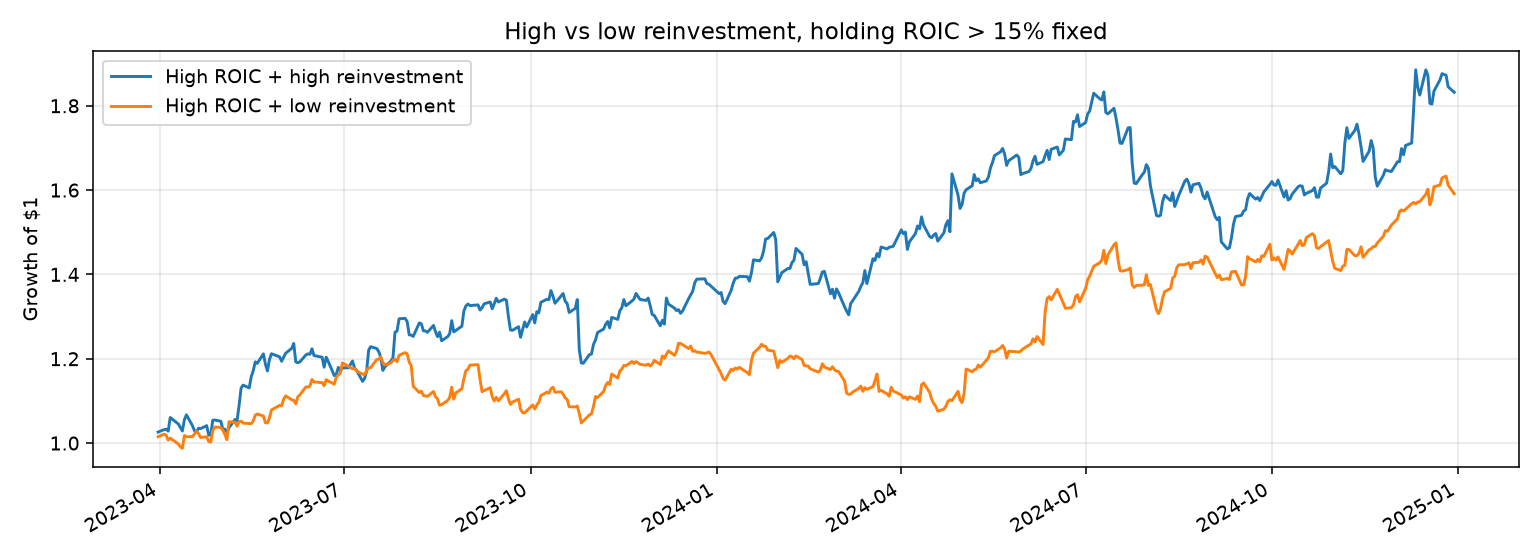
\includegraphics[width=0.88\textwidth]{figures/reinvestment-split.png}
\caption{High versus low reinvestment, holding ROIC $> 15\%$ fixed. The high-reinvestment sleeve pulls ahead through 2023--2024.}
\label{fig:reinv}
\end{figure}

\section{Attribution}
\label{sec:attrib}

Section~\ref{sec:results} shows that the book won on total return. This section asks whether that win looks like stock picking or like a hidden sector bet, especially the SaaS, healthcare, and med-tech tilt named in the original hypothesis.

\subsection{Alpha, beta, and tracking error}

Daily excess returns of the compounder book are regressed on each benchmark (CAPM-style, 2\% risk-free rate). Alpha is annualized.

\begin{table}[htbp]
\centering
\caption{Halal ROIC compounders versus each benchmark, live window.}
\label{tab:capm}
\begin{tabular}{lrrrrr}
\toprule
Benchmark & Alpha (ann.) & Beta & $R^2$ & Tracking error & Info.\ ratio \\
\midrule
S\&P~500     & 10.00\% & 1.18 & 0.72 & 10.68\% & 1.28 \\
Halal (SPUS) & 8.06\%  & 1.07 & 0.80 & 8.89\%  & 1.10 \\
\bottomrule
\end{tabular}
\end{table}

Versus SPY the book is more aggressive ($\beta = 1.18$) with 10.0\% leftover annualized alpha. Versus SPUS it is almost a parallel book: $\beta = 1.07$, $R^2 = 0.80$, still 8.1\% alpha. In other words, this is an SPUS-like Halal large-cap book with extra mega-cap platform exposure, not an independent style that moves on its own.

The information ratios (1.28 versus SPY, 1.10 versus SPUS) look respectable because the sample includes two strong years. They will shrink if a full down year such as 2022 is added.

\subsection{Focus-sector and GICS exposure}

Average month-end weights of the cap-weighted compounder book are compared with an equal-weight basket of the Halal S\&P universe.

\begin{table}[htbp]
\centering
\caption{Average focus-bucket weights. Delta is compounder book minus equal-weight Halal universe.}
\label{tab:focus}
\small
\begin{tabular}{lrrr}
\toprule
Bucket & Compounder book & Halal universe (EW) & Delta \\
\midrule
Other                      & 73.7\% & 77.7\% & $-4.0\%$ \\
SaaS                       & 16.6\% & 9.1\%  & $+7.5\%$ \\
Healthcare                 & 9.4\%  & 5.7\%  & $+3.7\%$ \\
MedTech                    & 2.0\%  & 7.5\%  & $-5.5\%$ \\
\bottomrule
\end{tabular}
\end{table}

SaaS and healthcare are overweights. Med-tech is an underweight. Cap-weighting Nvidia, Microsoft, Alphabet, and Meta leaves ``other'' at 74\% despite many tagged names in the high-ROIC pool.

\begin{figure}[htbp]
\centering
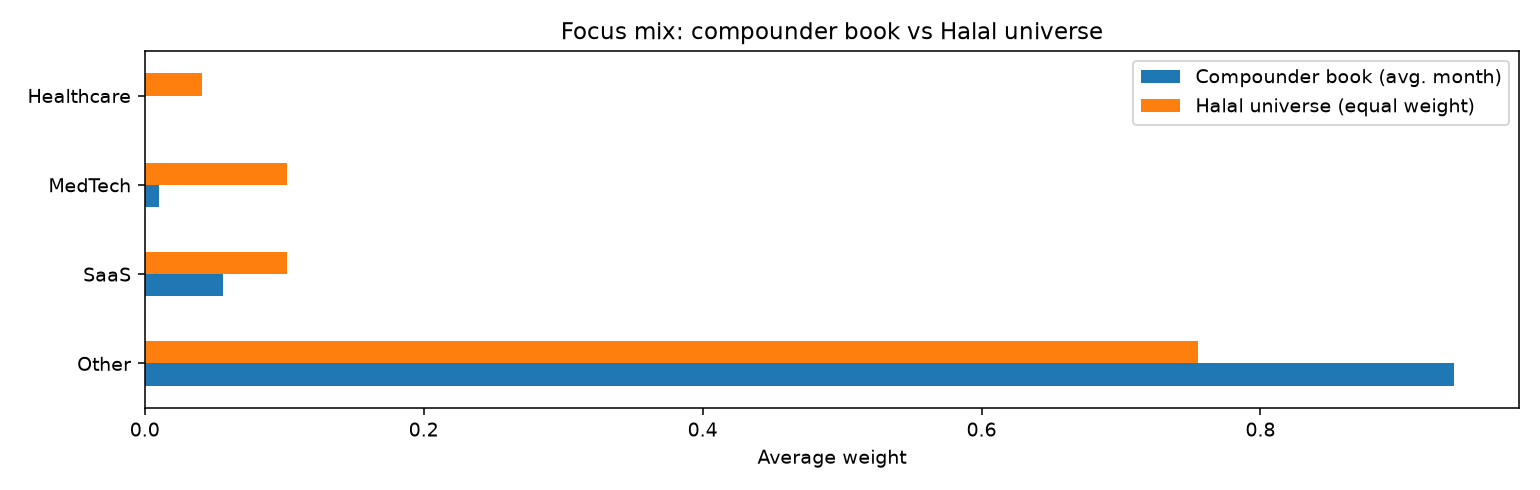
\includegraphics[width=0.88\textwidth]{figures/focus-mix.png}
\caption{Focus mix: compounder book versus equal-weight Halal universe. Med-tech is lighter than the universe, not heavier.}
\label{fig:focus}
\end{figure}

\begin{table}[htbp]
\centering
\caption{Average GICS sector weights. Delta is compounder book minus equal-weight Halal universe.}
\label{tab:sectors}
\small
\begin{tabular}{lrrr}
\toprule
Sector & Compounder book & Halal universe (EW) & Delta \\
\midrule
Technology                 & 44.6\% & 19.1\% & $+25.5\%$ \\
Communication services     & 37.8\% & 5.5\%  & $+32.4\%$ \\
Healthcare                 & 9.7\%  & 13.4\% & $-3.8\%$ \\
Consumer cyclical          & 6.8\%  & 11.6\% & $-4.8\%$ \\
Consumer defensive         & 5.5\%  & 6.4\%  & $-0.9\%$ \\
Energy                     & 2.7\%  & 4.8\%  & $-2.1\%$ \\
Industrials                & 1.9\%  & 14.4\% & $-12.4\%$ \\
Basic materials            & 1.1\%  & 4.6\%  & $-3.4\%$ \\
Utilities                  & 0.0\%  & 7.1\%  & $-7.1\%$ \\
Real estate                & 0.0\%  & 6.8\%  & $-6.8\%$ \\
Financial services         & 0.0\%  & 6.2\%  & $-6.2\%$ \\
\bottomrule
\end{tabular}
\end{table}

Technology plus communication services average 82.4\% of the book. Utilities, real estate, and financial services are empty. That is more concentrated than a diversified capital-light healthcare product, and more concentrated than the companion FCF-quality backtest in this series, where technology plus communication services averaged about 74\% of weight.

\begin{figure}[htbp]
\centering

\includegraphics[width=0.88\textwidth]{figures/sector-mix.png}
\caption{GICS sector mix: compounder book versus equal-weight Halal universe. The book is a platform and technology overweight, not a diversified capital-light healthcare book.}
\label{fig:sectors}
\end{figure}

\subsection{What can and cannot be isolated}

The leftover alpha versus SPUS is still positive after a $\beta \approx 1$ fit, so the result is not only a restatement of SPUS. SPUS itself is already Halal and tech-tilted in this window, and this book is more concentrated in the same mega-cap platform names.

The reinvestment split supports the engine part of the hypothesis: among high-ROIC Halal names, ploughing capital back in paid in 2022--2024. The sector part is weaker. Med-tech did not dominate, and the SaaS/healthcare/med-tech-only sleeve did not beat the main book.

Without a sector-neutral twin I cannot say how much of the 8\% SPUS alpha is reinvestment sorting versus even more Nvidia, Microsoft, Alphabet, and Meta than SPUS already owned. The fair reading is that reinvestment sorting inside a Halal high-ROIC pool produced a mega-cap platform book, and that book paid in 2022--2024.

\section{Limitations and implementation friction}
\label{sec:limits}

\subsection{Turnover, slippage, and net CAGR}

Turnover is one-way: half the $\ell_1$ weight change between consecutive month-end books. Trading-cost drag assumes 10~basis points per one-way turn.

\begin{table}[htbp]
\centering
\caption{Implementation friction on the live compounder book.}
\label{tab:friction}
\begin{tabular}{lr}
\toprule
Item & Value \\
\midrule
Rebalances with holdings              & 27 \\
Average names held                    & 47.6 \\
Annualized one-way turnover           & 200.2\% \\
Assumed cost per one-way trade        & 10~bp \\
Estimated annual trading-cost drag    & 0.20\% \\
CAGR gross of trading costs           & 39.57\% \\
CAGR net of trading costs             & 39.24\% \\
\bottomrule
\end{tabular}
\end{table}

Annualized one-way turnover of 200\% looks high because the book ramps from a thin early window and rebalances monthly across about 50 names. Cost drag at 10~bp is 20~bp a year, small next to the headline CAGR, though real slippage on smaller reinvestment picks could be wider. I do not model market impact, borrow, or taxes.

\begin{figure}[htbp]
\centering

\includegraphics[width=0.88\textwidth]{figures/turnover.png}
\caption{One-way turnover at each rebalance. Spikes appear when the book expands. Steady-state months are lower but not negligible.}
\label{fig:turnover}
\end{figure}

\subsection{Purification drag}

Impure income that may require purification is reported, not ignored. Using the library's dividend-purification helper on names that appeared in the book, there were 213 dividend events while held, and annualized purification drag is about 0.00\%. That is negligible next to 39.6\% CAGR. Missing interest-income tags are a gap, not evidence of zero drag.

\subsection{Point-in-time compliance}

Screens are applied at each rebalance. Failed names are sold then. There is no intra-month compliance monitor. Sector exclusions use the current S\&P list and current activity labels, not the 2019 membership file. That is survivorship and look-ahead in the universe, even though the filings themselves use \texttt{filed\_date}.

\subsection{Data and construction issues}

Yahoo annual statements typically store only a few years. The first metrics date is 30~November~2021 and the first invested date is 31~October~2022, so the 2019--2021 request is mostly unused. NOPAT, invested capital, CapEx, D\&A, $\Delta$NWC, and R\&D come from yfinance with a 90-day lag. Restatements and tag mapping are not audited here.

GOOG and GOOGL are both weighted, so Alphabet is overweight versus a single-listing index. There is no position cap, which means three names can be half the book. Many med-tech names failed the 15\% ROIC threshold on Yahoo data despite high reinvestment, so sector persistence cannot be read from weights alone. The 15\% ROIC threshold was fixed before the full run. It was not optimized on a hold-out, but the live window is short enough that any threshold choice is still partly in-sample.

\subsection{What this paper does not show}

There is no full calendar year 2022, no 2008, no rate-hike recession, and no hold-out after a rule freeze. ROIC quintiles are not monotonic. Sector mix explains a large part of the path. Beating SPUS in a mega-cap boom is interesting. It is not evidence that Halal ROIC compounders persist across cycles in capital-light sectors, which was the original question.

\section{Conclusion}
\label{sec:conc}

A cap-weighted book of AAOIFI-screened S\&P~500 names with ROIC above 15\% and high reinvestment rates beat SPY and SPUS from late 2022 through 2024. The more informative diagnostic is the reinvestment split inside that high-ROIC pool, not ROIC quintiles on their own. The live portfolio is still a concentrated Halal mega-cap technology and platform book. Restricting the same rule to SaaS, healthcare, and med-tech does not improve on SPUS.

The product shape is coherent enough to keep studying: Halal screens, a hard ROIC floor, a high-reinvestment cut, and cap-weighting. It is not ready to promote to a live mandate. A second paper would need a frozen rule, SEC income and cash-flow tags with a longer history, point-in-time S\&P membership, a single listing per issuer, a sector-capped or med-tech-inclusive twin with a ROIC definition that treats R\&D-heavy filers fairly, and at least one full down year. If the sector-capped twin still beats SPUS, the compounding claim has more to stand on. If it does not, the 40\% CAGR in this sample is mostly the 2023--2024 platform tape.

\paragraph{Reproduction.}
Run \texttt{code.ipynb} in this paper's folder with \texttt{FAST\_MODE=False} and dates 2019-01-01 to 2024-12-31. Figures are stored alongside the notebook. The public repository is \url{https://github.com/regional-specter/Monterey-Finance}.

\bibliographystyle{plainnat}
\begin{thebibliography}{9}

\bibitem[AAOIFI(2020)]{aaoifi21}
Accounting and Auditing Organization for Islamic Financial Institutions, 2020.
\newblock Financial Paper (Shares and Bonds).
\newblock Shari'ah Standard No.~21, AAOIFI, Manama.

\bibitem[Asness et~al.(2019)]{asness2019}
Asness, C.~S., Frazzini, A., Pedersen, L.~H., 2019.
\newblock Quality minus junk.
\newblock Review of Accounting Studies 24, 34--112.

\bibitem[Damodaran(2007)]{damodaran2007}
Damodaran, A., 2007.
\newblock Return on capital (ROC), return on invested capital (ROIC), and return on equity (ROE): Measurement and implications.
\newblock Working paper, Stern School of Business, New York University.

\bibitem[Derigs and Marzban(2008)]{derigs2008}
Derigs, U., Marzban, S., 2008.
\newblock Review and analysis of current Shariah-compliant equity screening practices.
\newblock International Journal of Islamic and Middle Eastern Finance and Management 1, 285--303.

\bibitem[Novy-Marx(2013)]{novymarx2013}
Novy-Marx, R., 2013.
\newblock The other side of value: The gross profitability premium.
\newblock Journal of Financial Economics 108, 1--32.

\bibitem[Peters and Taylor(2017)]{peters2017}
Peters, R.~H., Taylor, L.~A., 2017.
\newblock Intangible capital and the investment-$q$ relation.
\newblock Journal of Financial Economics 123, 251--272.

\end{thebibliography}

\end{document}
